\documentclass{beamer}

% \bibliographystyle{abbrv}
\setbeamertemplate{bibliography item}{\insertbiblabel}
  
\renewcommand{\footnotesize}{\tiny}
\setbeamerfont{framesubtitle}{size=\small}
\usepackage{url}



\usetheme{Warsaw}

%slides numbers
\addtobeamertemplate{navigation symbols}{}{%
    \usebeamerfont{footline}%
    \usebeamercolor[fg]{footline}%
    \hspace{1em}%
    \insertframenumber/\inserttotalframenumber
}

\title{Paying attention to Attention}
\author{Piotr Mazurek}
\centering
\date{\today}
\begin{document}
\maketitle



\begin{frame}{Agenda}
\begin{enumerate}


\item Introduction to Attention 

\item Introduction to Neural Networks

\item Basics of the Attention mechanism

\item Deep dive into Attention

\item Attention applications
 
\end{enumerate}
\end{frame}



\section{Introduction to attention}
\begin{frame}{Introduction to Attention}
\framesubtitle{Basic intuition}

\begin{figure}
    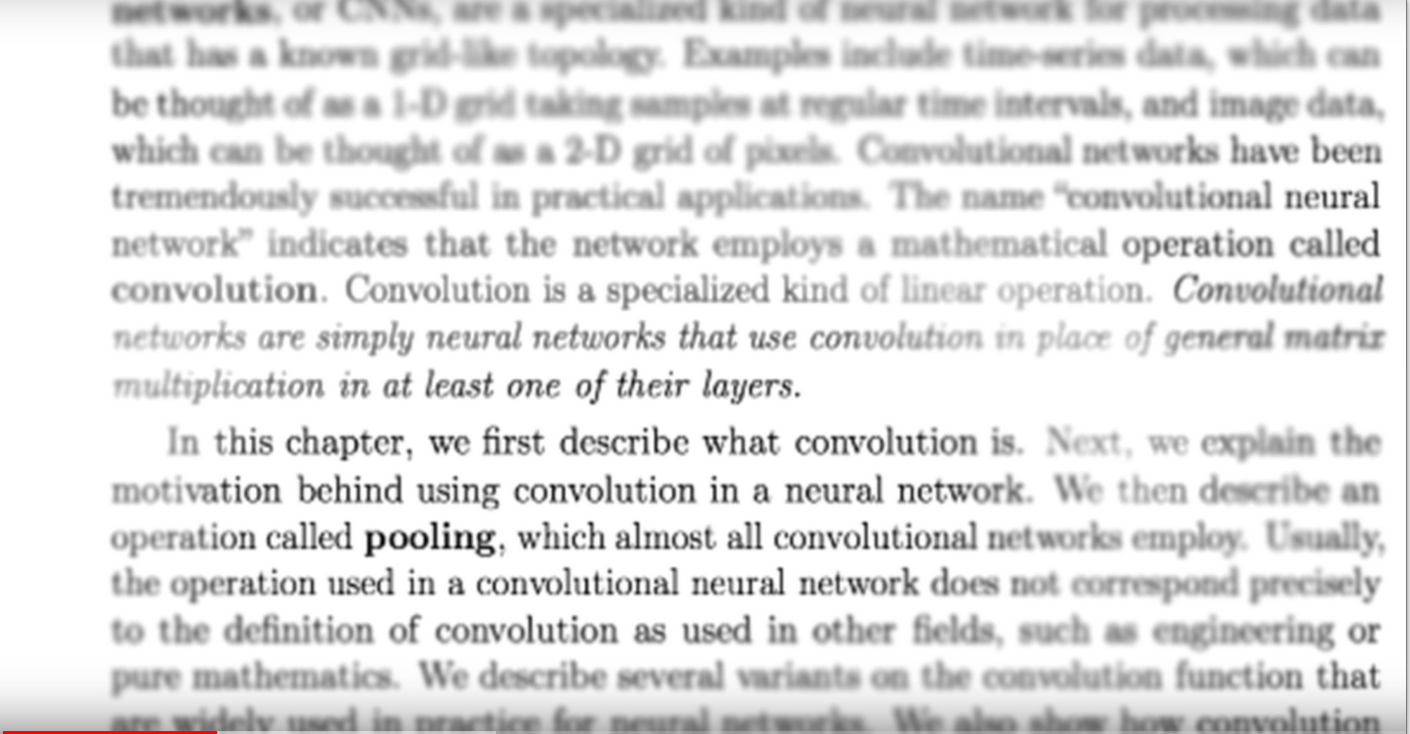
\includegraphics[width = .8\textwidth]{images/attention-intuition.png}
    \caption{We teach a neural network to focus on some part of the data\footnote{\url{https://www.youtube.com/watch?v=W2rWgXJBZhU&t=180s}}}
    % \label{fig:my_label}
\end{figure}{}

\end{frame}


\begin{frame}{Introduction to Attention}
\framesubtitle{Who, where and when?}

\begin{figure}
    \centering
    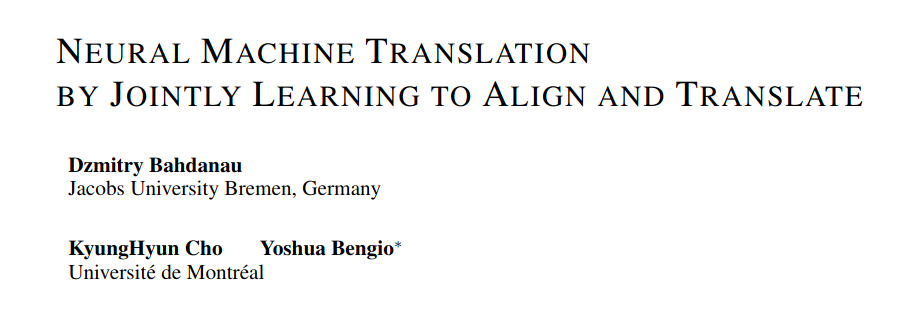
\includegraphics[width = .8\textwidth]{images/first-attention.png}
    \caption{Idea of the Attention first time mentioned (three times in the two consecutive lines, but still counts), Sept. 2014\cite{first-paper}}
    % \label{fig:my_label}
\end{figure}{}

\end{frame}


\begin{frame}{Introduction to Attention}
\framesubtitle{Who, where and when?}

\begin{figure}
    \centering
    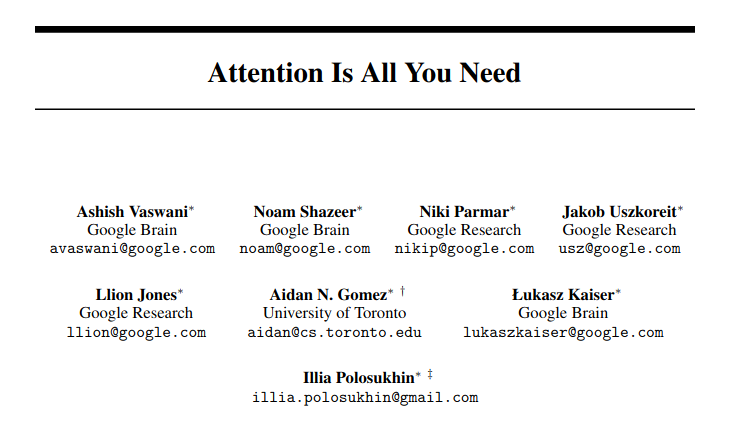
\includegraphics[width = .8\textwidth]{images/attention-is-all-you-need.png}
    \caption{Attention is all You need paper, Dec. 2017\cite{attention-is-all-you-need}}
    % \label{fig:my_label}
\end{figure}{}

\end{frame}



\begin{frame}{Introduction to Attention}
\framesubtitle{Boom in Attention papers}

\begin{figure}
    \centering
    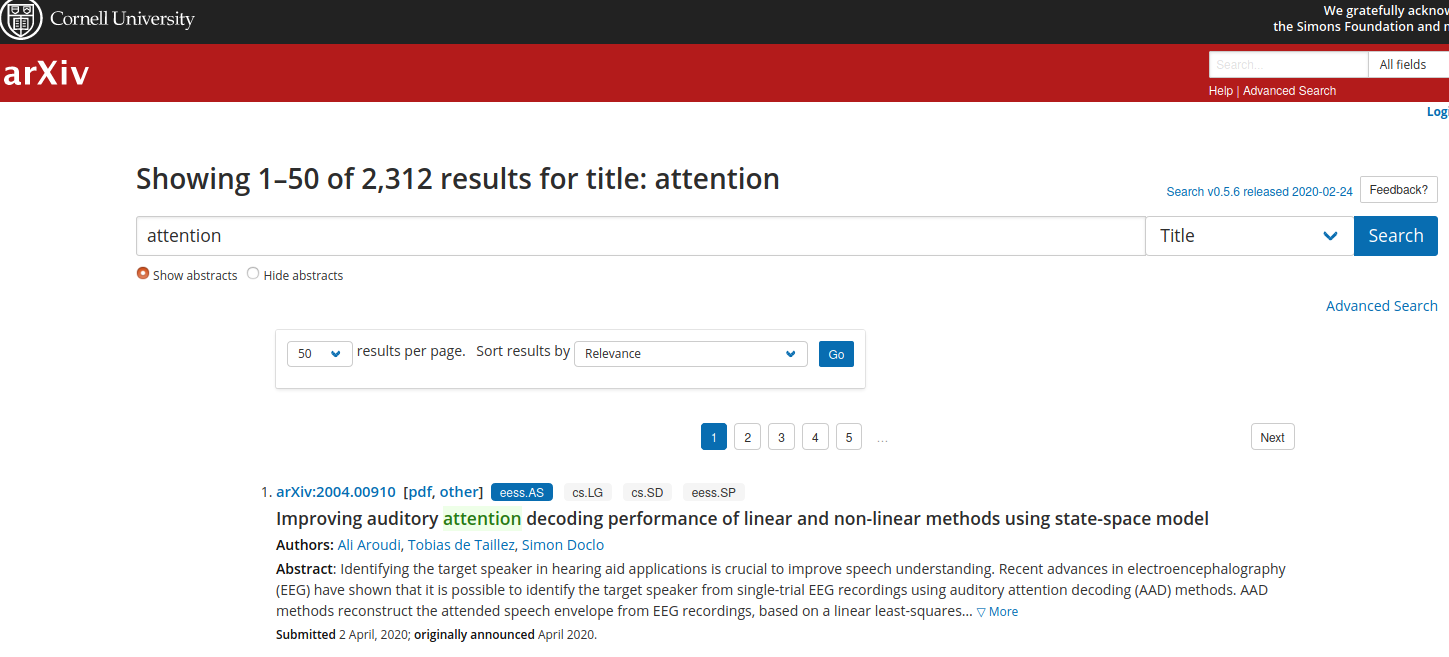
\includegraphics[width = .8\textwidth]{images/attention-arxiv.png}
    \caption{Attention - a hot research topic}
    % \label{fig:my_label}
\end{figure}{}

\end{frame}


\begin{frame}{Introduction to Attention}
\framesubtitle{Better start paying attention now}

\begin{figure}
    \centering
    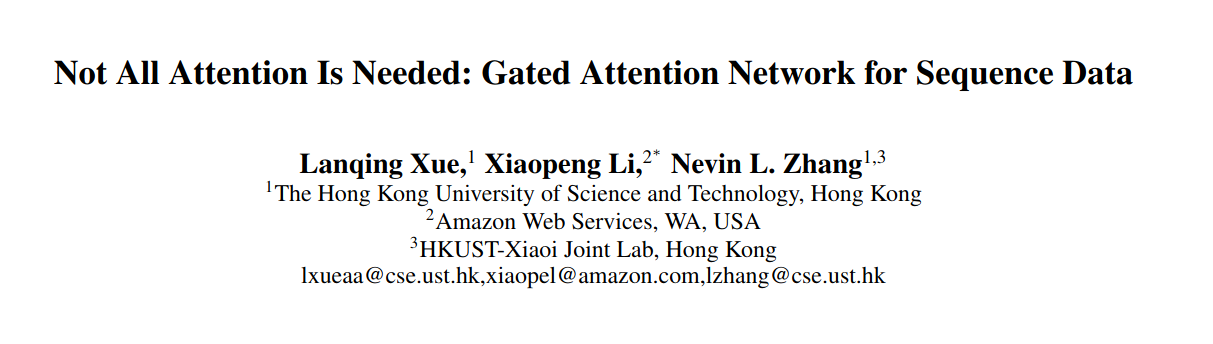
\includegraphics[width = .99\textwidth]{images/gated-attention.png}
    \caption{Not All Attention Is Needed, Dec. 2019}\cite{not-all-attention-is-neededr}
    % \label{fig:my_label}
\end{figure}{}

\end{frame}




\section{Introduction to Neural Networks}
\begin{frame}{Neural Networks - basic introduction}

\begin{figure}
    \centering
    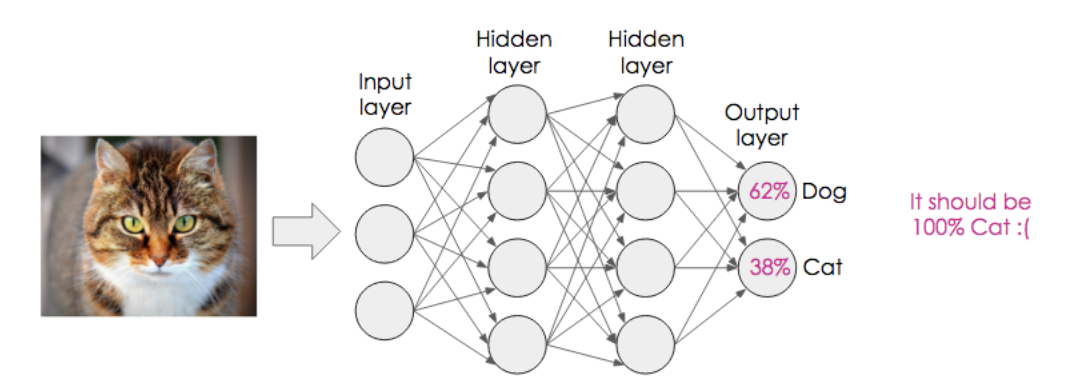
\includegraphics[width = .9\textwidth]{images/cat-neural-network.png}
    \caption{Not trained neural network\footnote{\url{https://www.fromthegenesis.com/artificial-neural-network-part-5/}}}
    % \label{fig:my_label}
\end{figure}{}

\end{frame}

\begin{frame}{Neural Networks}
\framesubtitle{Linear Algebra}
\begin{figure}
    \centering
    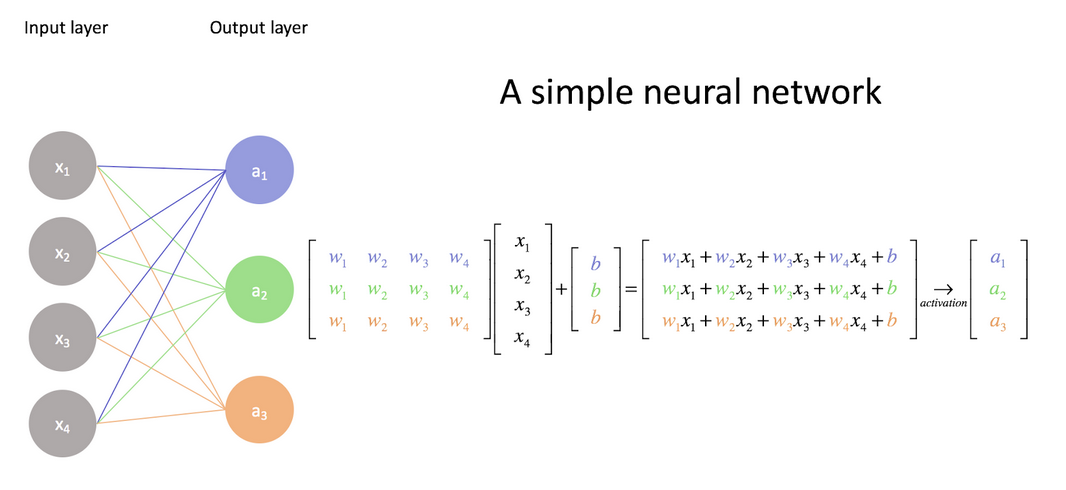
\includegraphics[width = .8\textwidth]{images/matrix.png}
    \caption{How matrices are used to compute values in neurons  \footnote{\url{https://www.jeremyjordan.me/intro-to-neural-networks/}}}
    % \label{fig:my_label}
\end{figure}{}
\end{frame}


\begin{frame}{Neural Networks}
\framesubtitle{Algebraic intuition}
\begin{figure}
    \centering
    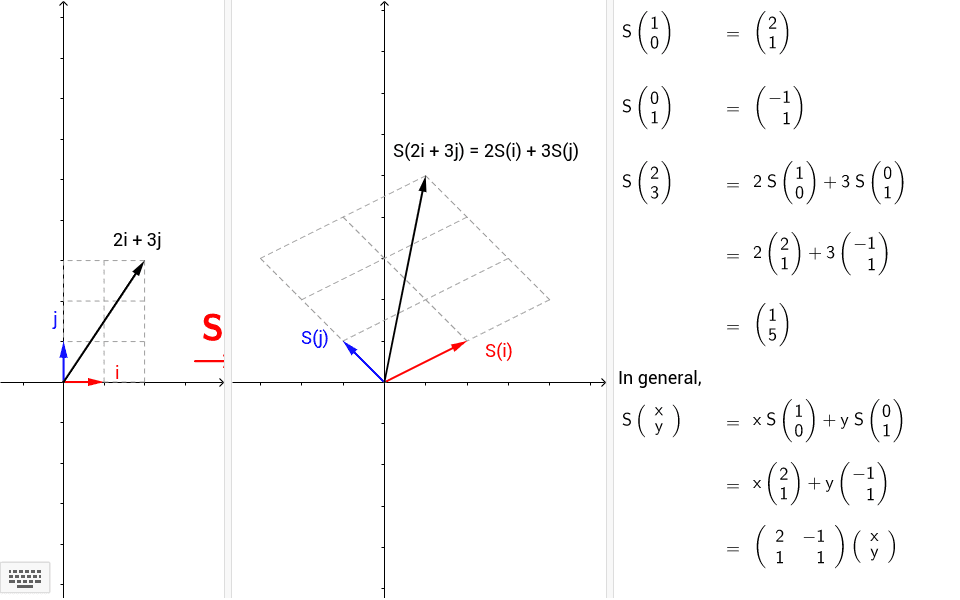
\includegraphics[width = .7\textwidth]{images/linear-transformation.png}
    \caption{Linear Transformation \footnote{\url{https://www.geogebra.org/m/B9Nbwh7w}}}
    % \label{fig:my_label}
\end{figure}{}
\end{frame}




\begin{frame}{Mathematical Formalization}
\framesubtitle{Oversimplified}
        \begin{block}{Neural network in general}
        \begin{equation}
        f(x, \theta) = \hat{y} 
        \end{equation}
        where:\\
        $x$: input data\\
        $\Theta$: model parameters\\ 
        $\hat{y}$: distribution of probability over set of classes
        \end{block}\pause
        
        \begin{block}{Example}
        \begin{equation}
        f(x, w, b) = \sigma (x^{T}w + b)
        \end{equation}
        \end{block}
\end{frame}


\begin{frame}{Loss Function}
\framesubtitle{How to find $\theta$}
        
        \begin{block}{How to find $\theta$}
        \begin{equation}
        \underset{\theta}{\text{minimize}} \: J(\theta)    
        \end{equation}{}
        
        For example we can use SGD optimizer 
        
        \end{block}\pause
        
        \begin{block}{Example loss function}
        \begin{equation}
        J(\theta)=\frac{1}{2} \mathbb{E}_{\mathbf{x}, \mathbf{y} \sim \hat{p}_{\mathrm{data}}}\|\boldsymbol{y}-f(\boldsymbol{x} ; \boldsymbol{\theta})\|^{2}
        \end{equation}
        \end{block}
\end{frame}

\begin{frame}{Latent space}
\framesubtitle{Auto-encoder}

\begin{figure}
    \centering
    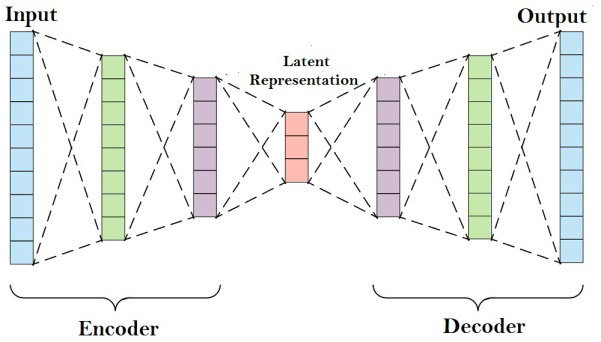
\includegraphics[width = .7\textwidth]{images/auto-encoder.jpg}
    \caption{Example auto-encoder\footnote{\url{https://towardsdatascience.com/applied-deep-learning-part-3-autoencoders-1c083af4d798}}}
    % \label{fig:my_label}
\end{figure}{}
    
\end{frame}

\begin{frame}{Latent space}
\framesubtitle{The big picture}



\begin{columns}
\begin{column}{0.5\textwidth}
    \begin{itemize}
    \item Used to find the hidden representation of data
    
    \item By training model on a particular set of data we create some kind of general knowledge
    
    \end{itemize}   
\end{column}
\begin{column}{0.5\textwidth}  %%<--- here
\begin{figure}
    \begin{center}
    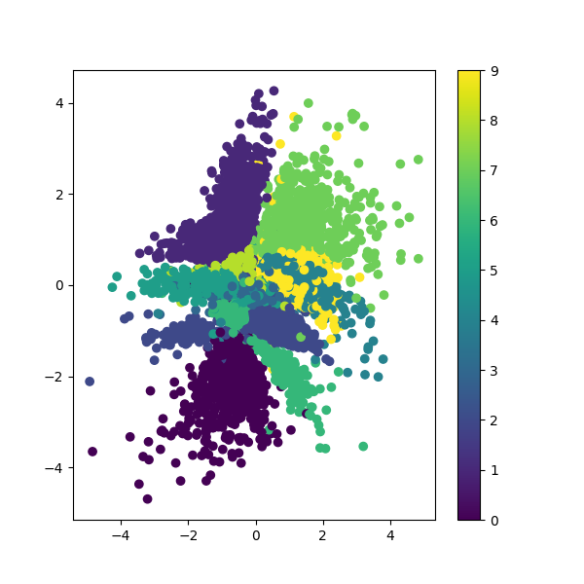
\includegraphics[width = .7\textwidth]{images/latent-space.png}
    \caption{Finding information in chaos}    
    \end{center}{}
    
    % \label{fig:my_label}
\end{figure}
\end{column}

\end{columns}
    
\end{frame}


\begin{frame}{Recurrent Neural Networks (RNNs)}
\framesubtitle{Oversimplified}


\begin{columns}
\begin{column}{0.5\textwidth}
    \begin{itemize}
    \item Used for sequential data. E.g for text analysis, video recognition etc.\pause
    
    \item Have so-called "local memory" or "state memory"\pause

    \item Computationally expensive to train\pause
    
    \item Problems with vanishing gradient\pause
    
    
    \end{itemize}   
\end{column}
\begin{column}{0.5\textwidth}  %%<--- here
    \begin{figure}
        \centering
        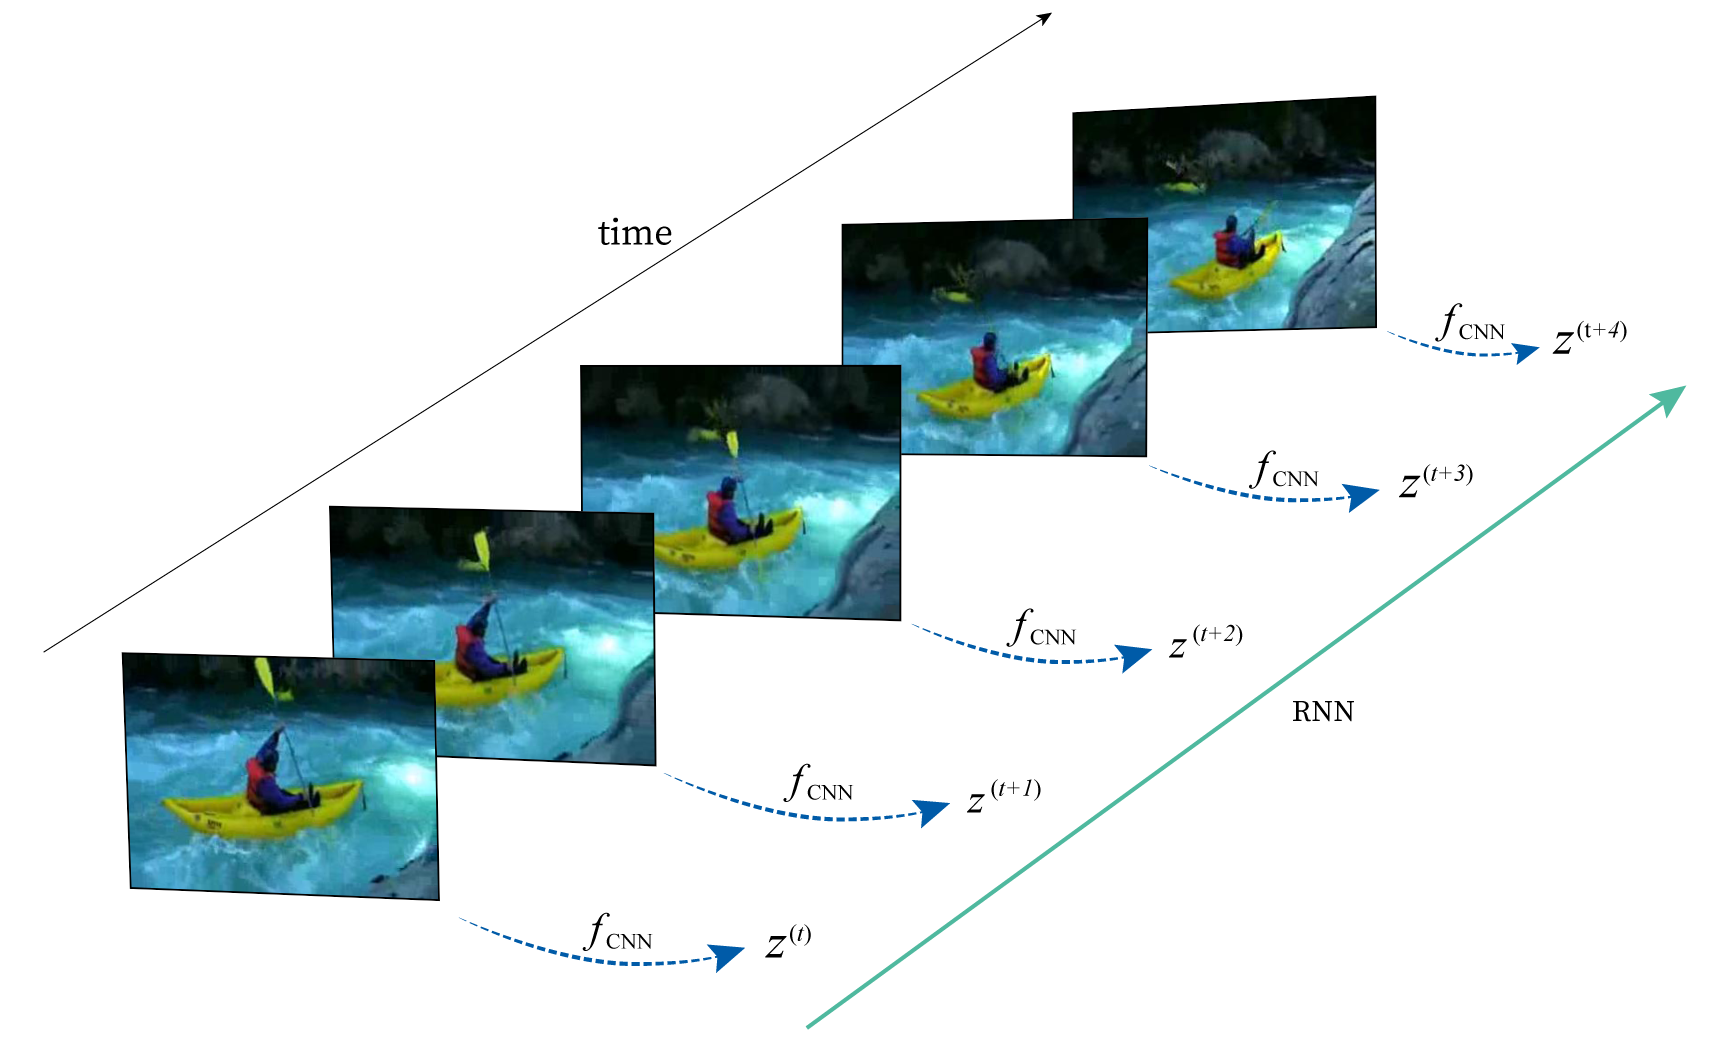
\includegraphics[width=0.8\textwidth]{images/CRNN.png}
        \caption{Sequence of frames\footnote{\url{https://awesomeopensource.com/project/HHTseng/video-classification}}}
        % \label{fig:my_label}
    \end{figure}{}
\end{column}
\end{columns}

{}
    
\end{frame}


\begin{frame}{Recurrent Neural Networks (RNNs)}
\framesubtitle{Oversimplified}

\begin{figure}
    \centering
    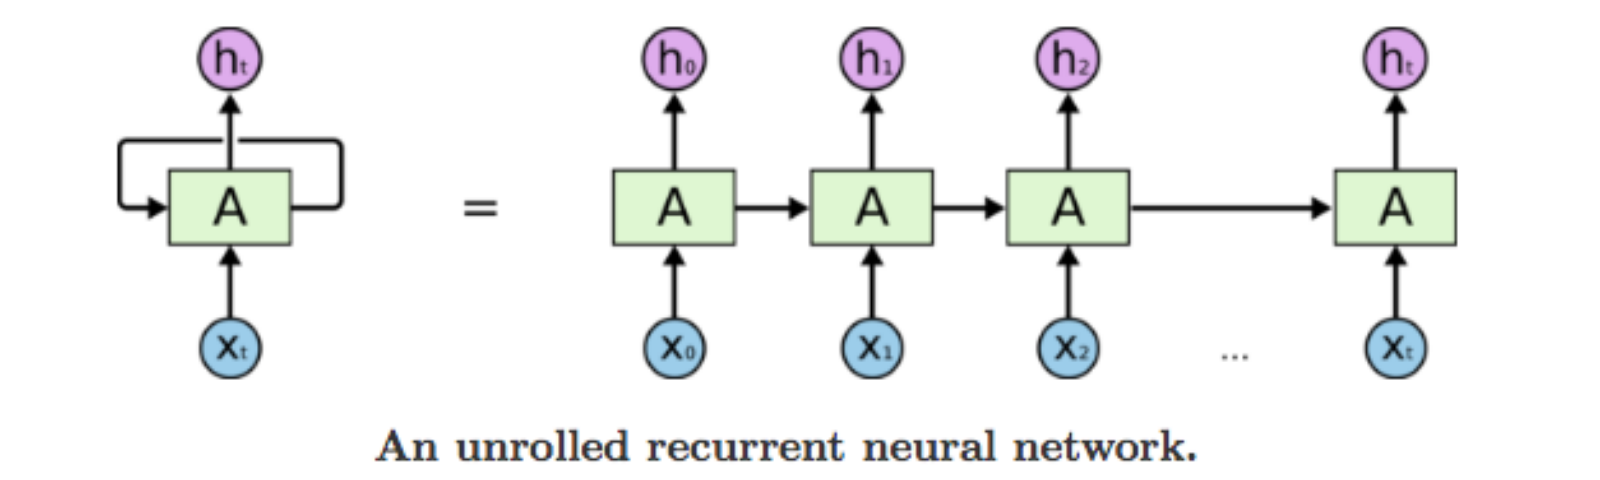
\includegraphics[width = .7\textwidth]{images/rnn.png}
    \caption{Folded and unfolder RNN \footnote{\url{https://towardsdatascience.com/understanding-rnn-and-lstm-f7cdf6dfc14e}}}
    % \label{fig:my_label}
\end{figure}{}
    
\end{frame}




\begin{frame}{Types of RNN}
\framesubtitle{Vector to sequence model}
\begin{figure}
    \centering
    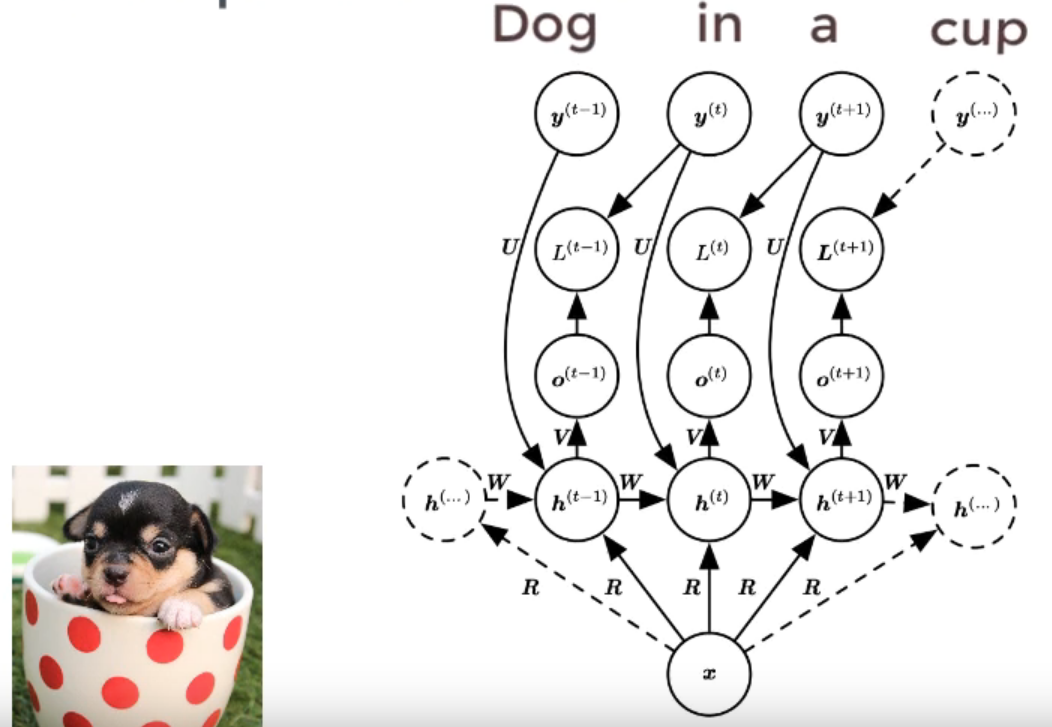
\includegraphics[width = .6\textwidth]{images/vec-2-sec.png}
    \caption{From an image (vector) generate a caption(sequence) \footnote{\url{https://www.youtube.com/watch?v=TQQlZhbC5ps&t=610s}}}
    % \label{fig:my_label}
\end{figure}{}
    
\end{frame}




\begin{frame}{Types of RNN}
\framesubtitle{Sequence to vector model}
\begin{figure}
    \centering
    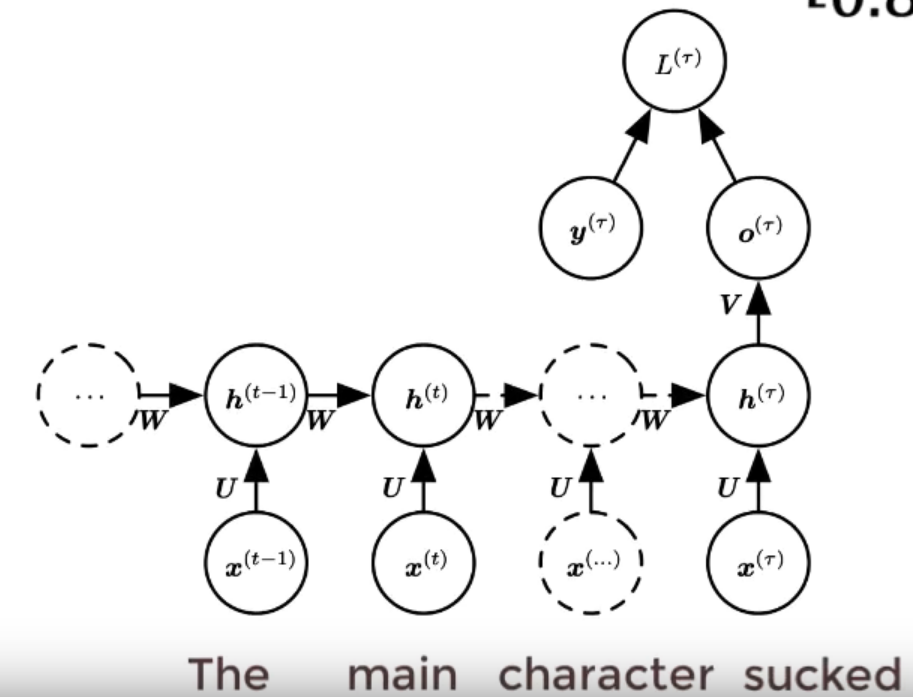
\includegraphics[width = .5\textwidth]{images/seq-2-vec.png}
    \caption{Take a review (sequence) and predict whether it is positive or negative (vector)\footnotemark[7]
    }
    % \label{fig:my_label}
\end{figure}{}
    
\end{frame}

\begin{frame}{Types of RNN}
\framesubtitle{Sequence to sequence (seq2seq) model}
\begin{figure}
    \centering
    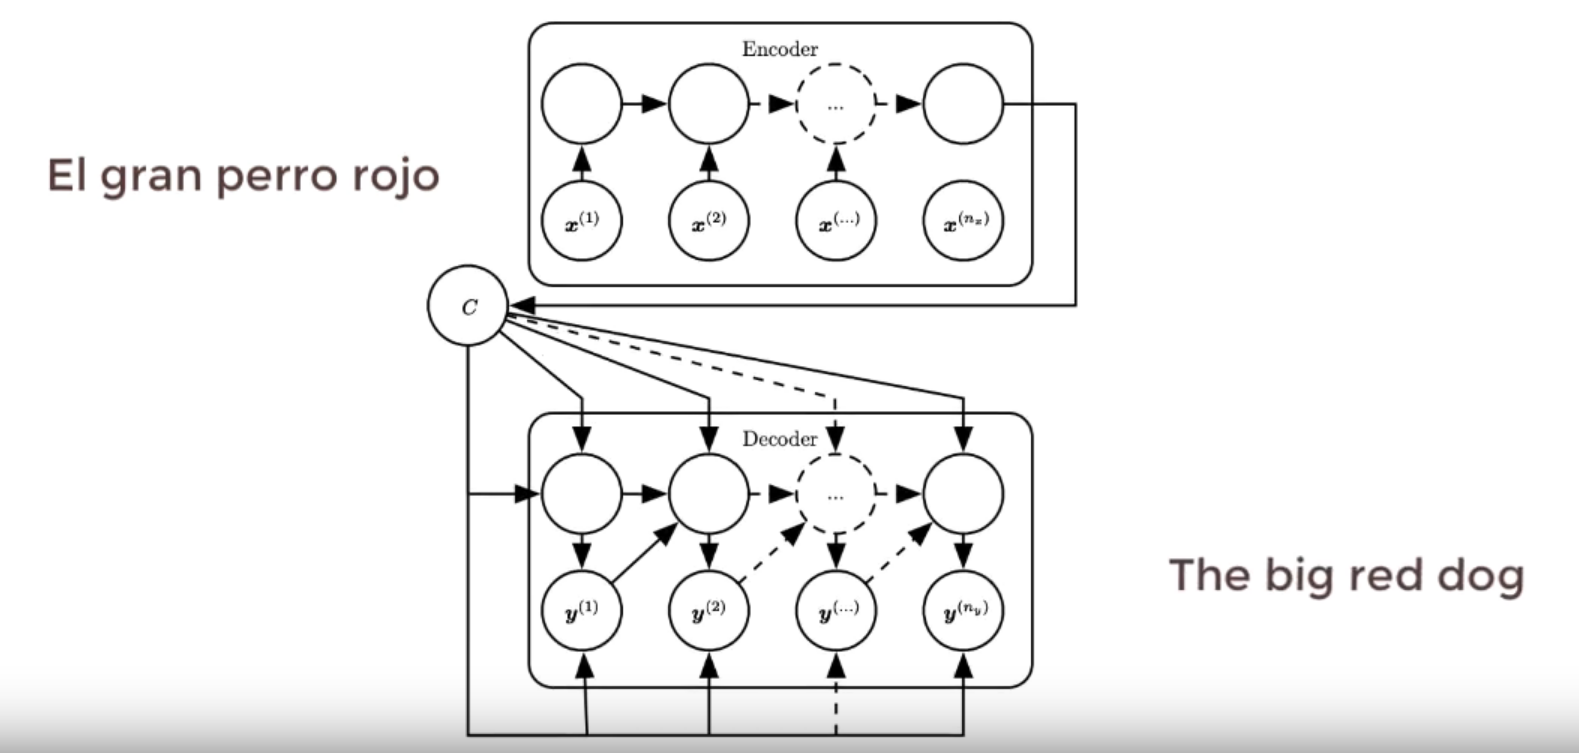
\includegraphics[width = .6\textwidth]{images/seq-2-seq.png}
    \caption{Translate a sentence in Spanish (sequence) into a sentence in English (sequence)\footnotemark[7]
    }
    % \label{fig:my_label}
\end{figure}{}
    
\end{frame}



\section{Introduction to attention mechanism}
\begin{frame}{Attention basic concept - recap}
\begin{figure}
    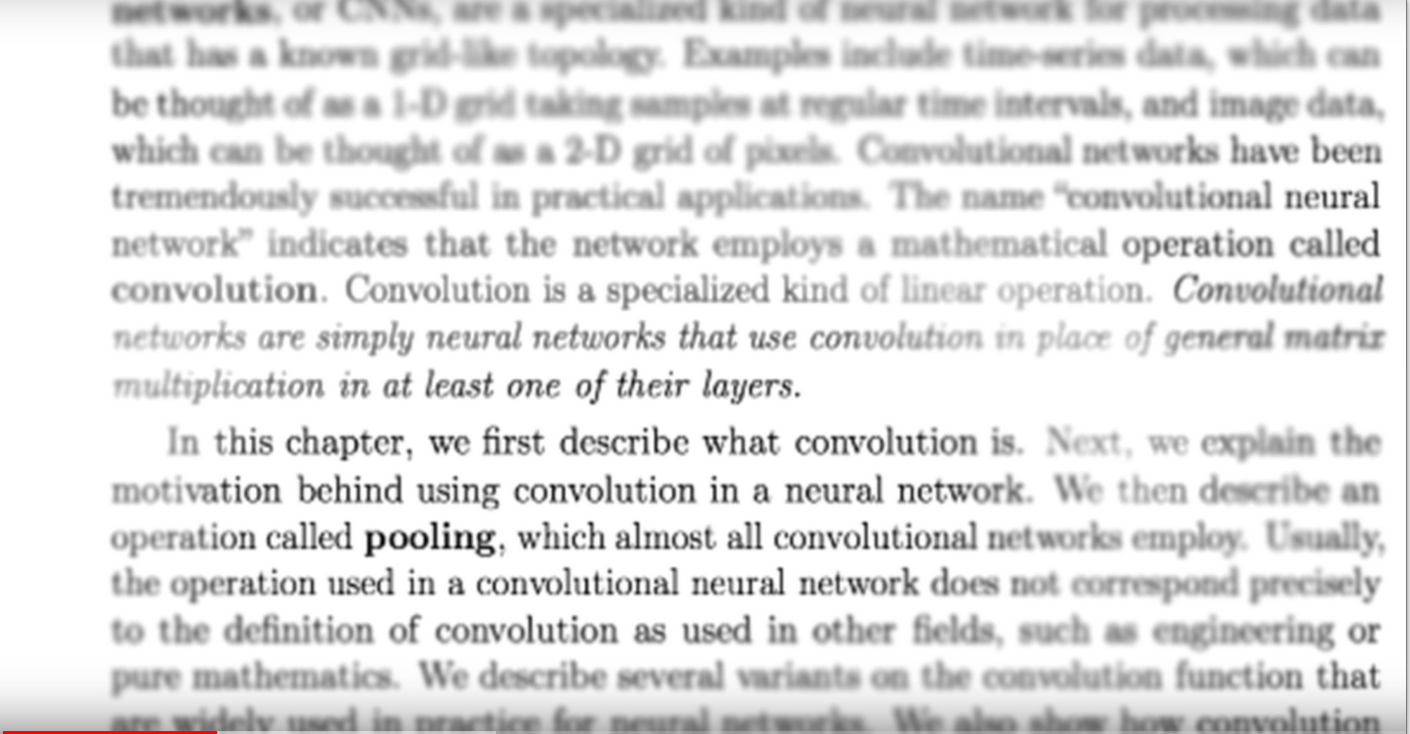
\includegraphics[width = .8\textwidth]{images/attention-intuition.png}
    \caption{We teach a neural network to focus on the part of the data\footnotemark[1]}
    % \label{fig:my_label}
\end{figure}{}
    
\end{frame}


\begin{frame}{Attention basic framework}
\framesubtitle{EEAP}
\begin{center}
\begin{enumerate}
    \item Embed\pause
    
    \item Encode\pause
    
    \item Attend\pause
    
    \item Predict
\end{enumerate}{}
\end{center}{}    
\end{frame}

\section{Deep dive into attention}


\begin{frame}{Pet problem to work with}
\framesubtitle{Encoder}
    \begin{figure}
    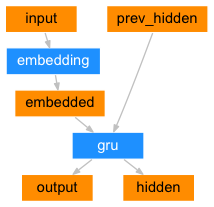
\includegraphics[width = .4\textwidth]{images/encoder-network.png}
    \caption{Our encoder model\footnote{\url{https://pytorch.org/tutorials/intermediate/seq2seq_translation_tutorial.html}}}
    % \label{fig:my_label}
\end{figure}{}
\end{frame}

\begin{frame}{Pet problem to work with}
\framesubtitle{Attention}

\begin{columns}
\begin{column}{0.5\textwidth}
    \begin{itemize}
    \item We calculate attention weights based on \textbf{decoder input} and a hidden state
    
    \item We multiply it with \textbf{encoder outputs} to create a weighted combination
    
    \item It will help the decoder to "find out" which part of encoder output is "responsible" for which part of decoder output  
    
    \end{itemize}   
\end{column}
\begin{column}{0.5\textwidth}  %%<--- here
\begin{figure}
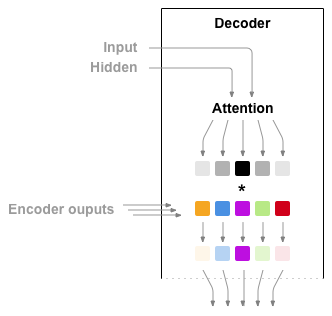
\includegraphics[width = .9\textwidth]{images/attention-weights.png}
\caption{Way of computing attention\footnotemark[8]}
\end{figure}{}
\end{column}
\end{columns}


\end{frame}


\begin{frame}{Pet problem to work with}
\framesubtitle{Decoder}
    \begin{figure}
    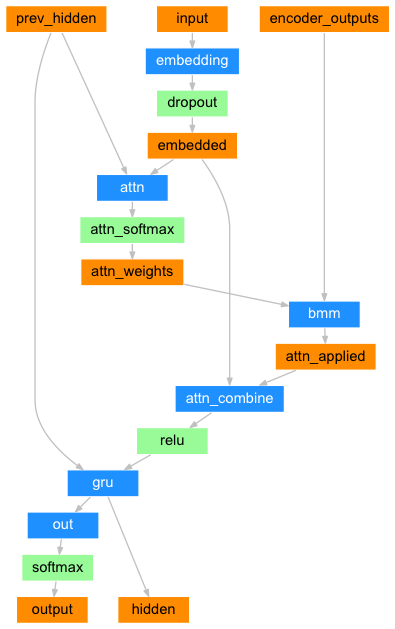
\includegraphics[width = .3\textwidth]{images/attention-decoder-network.png}
    \caption{Our attention-decoder model\footnotemark[8]}
    % \label{fig:my_label}
\end{figure}{}
\end{frame}


\begin{frame}{Time to code}

Now we will do a little bit of live coding

\begin{block}{Where can You find the code?}

\url{https://github.com/tugot17/paying-attention-to-attention}

\end{block}

    
\end{frame}

\section{Attention applications}



\begin{frame}{Attention applications}
\framesubtitle{Automatic image captioning}

\begin{columns}
\begin{column}{0.4\textwidth}
    \begin{itemize}
    \item Nearly the same solution as previously
    
    \item Instead of encoder output, latent space from a pre-trained state-of-the-art network (e.g Inception V3)
    
    \item Attention method similar as before (e.g Bahdanau Attention)
    
    \end{itemize}   
\end{column}
\begin{column}{0.7\textwidth}  %%<--- here
\begin{figure}
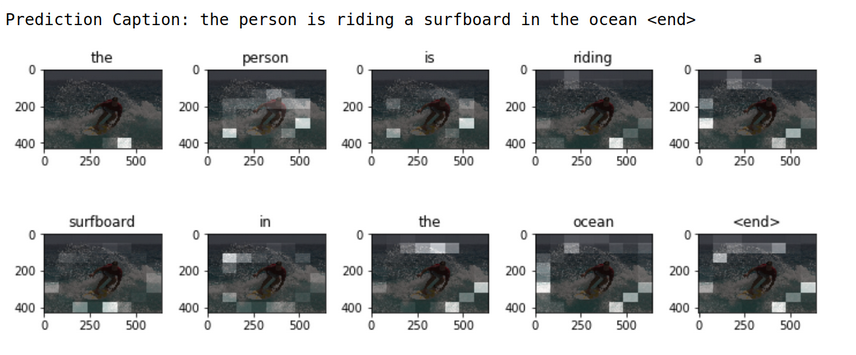
\includegraphics[width = .9\textwidth]{images/automatic-captions.png}
\caption{Show, Attend and Tell: Neural Image Caption Generation with Visual Attention\cite{image-caption}}
\end{figure}{}
\end{column}
\end{columns}
    
\end{frame}

\begin{frame}{Attention applications}
\framesubtitle{Attention UNet}

\begin{columns}
\begin{column}{0.4\textwidth}
    \begin{itemize}
    \item State-of-the-art image segmentation solution
    
    \item Improving model sensitivity and accuracy by attaching attention gates on top of the standard U-Net
    
    \end{itemize}   
\end{column}
\begin{column}{0.6\textwidth}  %%<--- here
\begin{figure}
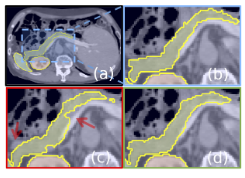
\includegraphics[width = .9\textwidth]{images/unet.png}
\caption{Segmentation for medical images with U-Net\cite{unet}}
\end{figure}{}
\end{column}
\end{columns}

    
\end{frame}


\begin{frame}{Attention applications}
\framesubtitle{Latex code generation}


\begin{columns}
\begin{column}{0.4\textwidth}
    \begin{itemize}
    \item Seq2seq very similar to the Image Captioning
    
    \item Uses attention based RNN to generate Latex Code
    
    \item Real world application: \url{https://mathpix.com/}
    
    \end{itemize}   
\end{column}
\begin{column}{0.6\textwidth}  %%<--- here
\begin{figure}
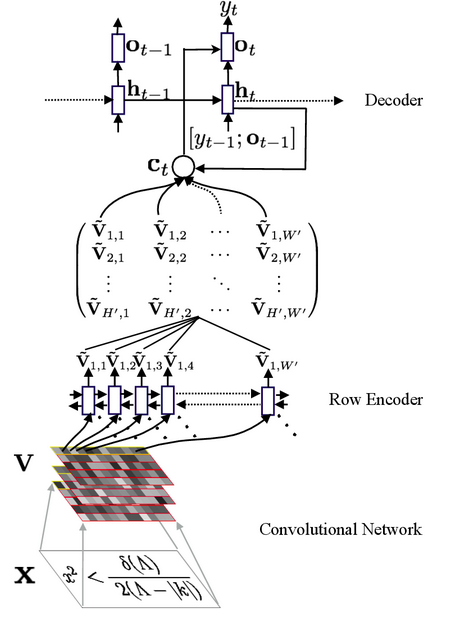
\includegraphics[width = .5\textwidth]{images/im-2-latex.png}
\caption{What You Get Is What You See:A Visual Markup Decompiler\cite{markup-decompiler}}
\end{figure}{}
\end{column}
\end{columns}

    
\end{frame}


\begin{frame}{Attention applications}
\framesubtitle{Many others, mainly some kind of seq2seq models}

\begin{columns}
\begin{column}{0.5\textwidth}
    \begin{itemize}
    \item Bert\cite{bert}, RoBerta\cite{roberta}, AlBert\cite{albert}, *Bert*
    
    \item GPT 2\cite{gpt2}
    
    \item Transformer - Attention is all You need\cite{attention-is-all-you-need} 
    
    \end{itemize}   
\end{column}
\begin{column}{0.5\textwidth}
    \begin{itemize}
    \item Residual Attention Network for Image Classification\cite{res-attention}
    
    \item TreeGen: A Tree-Based Transformer Architecture for Code Generation\cite{treegen}
    
    \item and many others ...
    
    
    \end{itemize} 

\end{column}
\end{columns}
    
\end{frame}


\section{Summary}
\begin{frame}{Summary}
\framesubtitle{Many others, mainly some kind of seq2seq models}

\begin{columns}
\begin{column}{0.5\textwidth}
    \begin{itemize}
    \item Attention = teach Your NN to on what part of data should it be focused on\pause
    
    \item Attention is all You need - we can solve a wide variety of problems using attention \pause
    
    \item We can use nearly same solution for many problems\pause
    
    \end{itemize}   
\end{column}
\begin{column}{0.5\textwidth}
    \begin{itemize}
    \item Embed, Encode, Attend, Predict Framework\pause
    
    \item Hot research topic - It's hard to stay up to date but it is relatively easy to publish\pause
    
    
    \item There are several methods for calculating attention (e.g Bahdanau Attention, Luong attention, etc.)
    
    \end{itemize} 

\end{column}
\end{columns}
    
\end{frame}


\begin{frame}[allowframebreaks]
        \frametitle{References}
        \bibliographystyle{plain}
        \bibliography{references.bib}
\end{frame}





\begin{frame}
\huge{\centerline{Thank You for Your attention}}
\end{frame}

\end{document}
